\chapter{Testy}
\label{cha:testy}

Sterowanie za pomocą komend głosowych może stać się o wiele cięższe w wykonaniu, kiedy w grę wchodzą czynniki takie jak akcent, inny niż stosowany w algorytmie język, dźwięki w tle, złożoność polecenia czy nawet niewyraźna mowa. Z uwagi na ten fakt, algorytm do rozpoznawania mowy używany w programie został poddany scenariuszom testowym. 

Na potrzeby testów przy użyciu darmowego narzędzia do generacji mowy \cite{conv} stworzono pięć zestawów tych samych dziesięciu poleceń widocznych w Tabeli \ref{tab:commands_test}, różniących się pomiędzy sobą kilkoma czynnikami:
\begin{itemize}
    \item oryginalny zestaw komend w języku angielskim z akcentem amerykańskim \textit{[EN]},
    \item wersja w języku angielskim z akcentem amerykańskim, gdzie prędkość nagrania to 2.0 \textit{[EN-0-2]},
    \item wersja w języku angielskim z akcentem Indii \textit{[EN-IN]},
    \item wersja w języku angielskim z akcentem Hong Kongu, gdzie prędkość nagrania to 0.5, a tonacja wyższa o 20 od normalnej \textit{[EN-HK-20-05]},
    \item wersja w języku polskim \textit{[PL]}.
\end{itemize}
            
\begin{center}
    \captionof{table}{Komendy użyte do testów.}
    \begin{tabular}{ |c|c|c| } 
    \hline
    Język & angielski & polski \\
    \hline
    \multirow{10}{4em}{Komenda} & spin in place & obróć się w miejscu \\ 
    & go forward & jedź naprzód \\ 
    & stop & zatrzymaj się \\ 
    & go backward & jedź do tyłu \\ 
    & speed 0.5 & prędkość 0.5 \\ 
    & start moving forward & zacznij ruch \\ 
    & go backward and turn right & jedź do tyłu i skręć w prawo \\ 
    & go backward and turn left & jedź do tyłu i skręć w lewo \\ 
    & go forward and turn right & jedź do przodu i skręć w prawo \\ 
    & go forward and turn left & jedź do przodu i skręć w lewo \\ 
    \hline
    \end{tabular}
    \label{tab:commands_test}
\end{center}

Do zestawów danych została dołożona również wersja polska, celem sprawdzenia użyteczności algorytmu w wypadku implementacji na fizycznym urządzeniu. Modyfikacje prędkości, tonacji i akcentów zostały wykonane na potrzeby zróżnicowania danych i wprowadzenia trudności dla algorytmu do zrozumienia komend. 

Używając metryki WER \ref{eq:wer} została obliczona średnia wartość błędu dla każdego z zestawów danych, widoczna na wykresie \ref{fig:dts1}. Można na nim zauważyć, że zgodnie z oczekiwaniami, zestaw \textit{[EN]} oryginalnych komend w języku angielskim posiada najmniejszą wartość błędu. Zarówno zestaw z akcentem Indii \textit{[EN-IN]} jak ten z akcentem Hong Kongu radzą sobie równie dobrze. Najbardziej wyróżnia się zestaw komend po polsku \textit{[PL]}, ze względu na niewystępujące w transkrypcji znaki łacińskie.

\begin{center}
    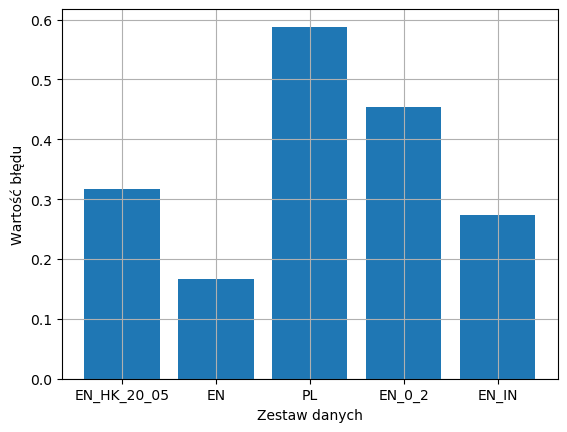
\includegraphics[width=0.95\linewidth]{files/output1.png}
    \captionof{figure}{Średnia wartość błędu.}
    \label{fig:dts1}
\end{center}

Po uwzględnieniu w transkrypcji znaków łacińskich, można zauważyć na wykresie \ref{fig:dts2} znaczny spadek wartości błędu dla zestawu komend w języku polskim. Potwierdza to użyteczność wykorzystywanego algorytmu do rozpoznawania mowy również poza środowiskiem testowym.

\begin{center}
    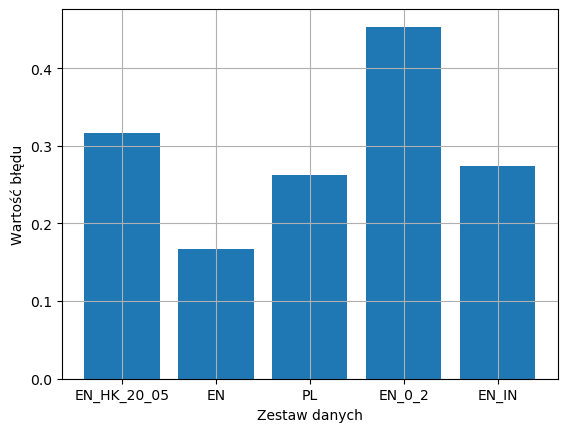
\includegraphics[width=0.95\linewidth]{files/output2.png}
    \captionof{figure}{Średnia wartość błędu po uwzględnieniu znaków łacińskich.}
    \label{fig:dts2}
\end{center}

% \break

Dane w zestawach widocznych w Tabeli \ref{tab:commands_test} dzielą się na dwie kategorie pod względem długości polecenia:
\begin{itemize}
    \item proste komendy, zawierające polecenie jednoargumentowe \textit{[komendy krótkie]},
    \item złożone komendy, zawierające polecenie dwuargumentowe \textit{[komendy długie]}.
\end{itemize}

Wśród krótkich komend można znaleźć polecenia jazdy do przodu, do tyłu, zatrzymania się czy ustawienia prędkości, natomiast wśród długich polecenia jazdy ze skrętem w różne strony. Na wykresie \ref{fig:dts3} można zauważyć znaczącą przewagę w rozpoznawaniu przez algorytm bardziej złożonych komend. Jest to prawdopodobnie spowodowane za dużą prostotą krótkich komend - część z nich to maksymalnie dwa słowa, które bez dalszego kontekstu są niezrozumiałe dla algorytmu i nie jest w stanie on określić ich znaczenia. 

Aby zagłębić się w strukturę czytelności poleceń, dla zestawów danych w języku angielskim z modyfikacjami została obliczona również średnia wartość błędu dla każdej z komend, która może zostać odczytana z wykresu \ref{fig:dts4}. Dla porównania, na wykresie została umieszczona również wartość błędu dla oryginalnego zestawu poleceń w języku angielskim.

\begin{center}
    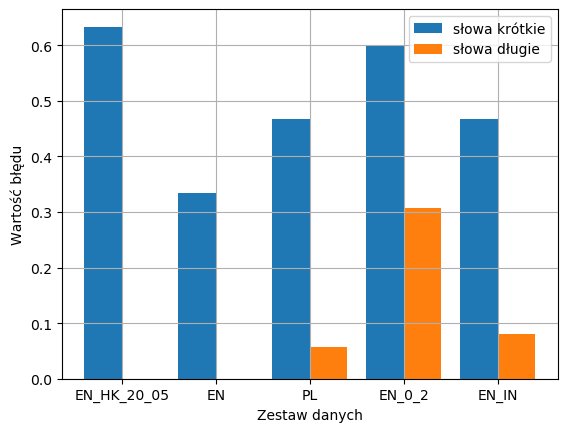
\includegraphics[width=0.8\linewidth]{files/output3.png}
    \captionof{figure}{Średnia wartość błędu dla komend krótkich i długich.}
    \label{fig:dts3}
\end{center}

\begin{center}
    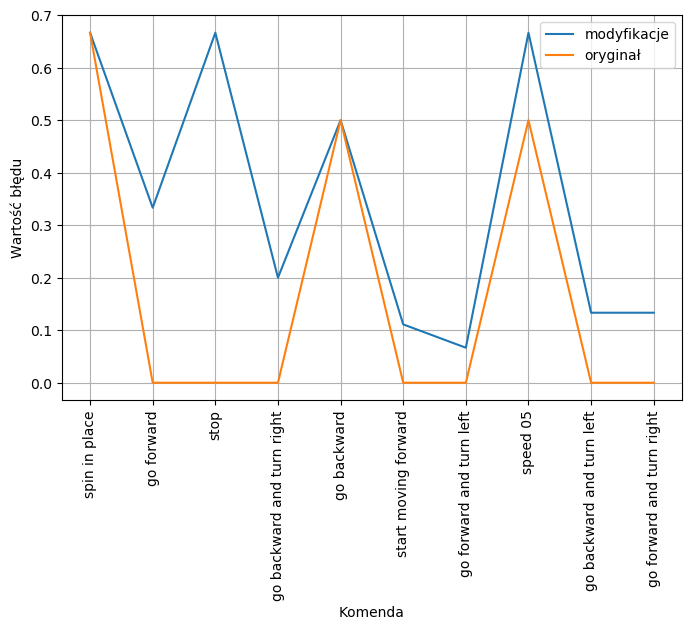
\includegraphics[width=0.8\linewidth]{files/output5.png}
    \captionof{figure}{Średnia wartość błędu dla każdej z komend.}
    \label{fig:dts4}
\end{center}

Jak wspomniano wcześniej, można zaobserwować znaczącą różnicę w rozpoznawalności krótkich poleceń, jak na przykład \textit{stop}, polecenie posiadające najwyższą średnią wartość błędu - niezrozumienia przez algorytm. W takim przypadku nierozpoznania polecenia, zostało zaimplementowane zabezpieczenie w postaci przełączenia robota w symulacji w tryb oczekiwania i ponowienie zapytania użytkownika o wydanie polecenia. 

Analizując wykres można dojść do wniosku, że algorytm w miarę sprawnie radzi sobie z rozpoznawaniem mowy nawet jeśli jest ona zmodyfikowana w jakiś sposób. Pomimo, że jest to bardzo mała próbka zestawu danych i może nie dostarczać w pełni wiarygodnych wyników, jednak spełnia aktualne potrzeby programu.

\vspace{10mm}

Drugim z przeprowadzonych testów był test spójności rozpoznawania mowy z obiektem w symulacji. Uruchomiono program widoczny na Rys.  \ref{fig:start_gazebo}, a następnie przy użyciu panelu do sterowania algorytm do rozpoznawania mowy z pliku. Na Rys. \ref{fig:ruch_gazebo} widoczna jest informacja zwrotna na panelu o rozpoznanej komendzie. Naciśnięcie drugi raz przycisku do rozpoznawania mowy powoduje zatrzymanie robota, a ponowne kliknięcie - ponowne uruchomienie algorytmu do rozpoznawania mowy.

\begin{center}
    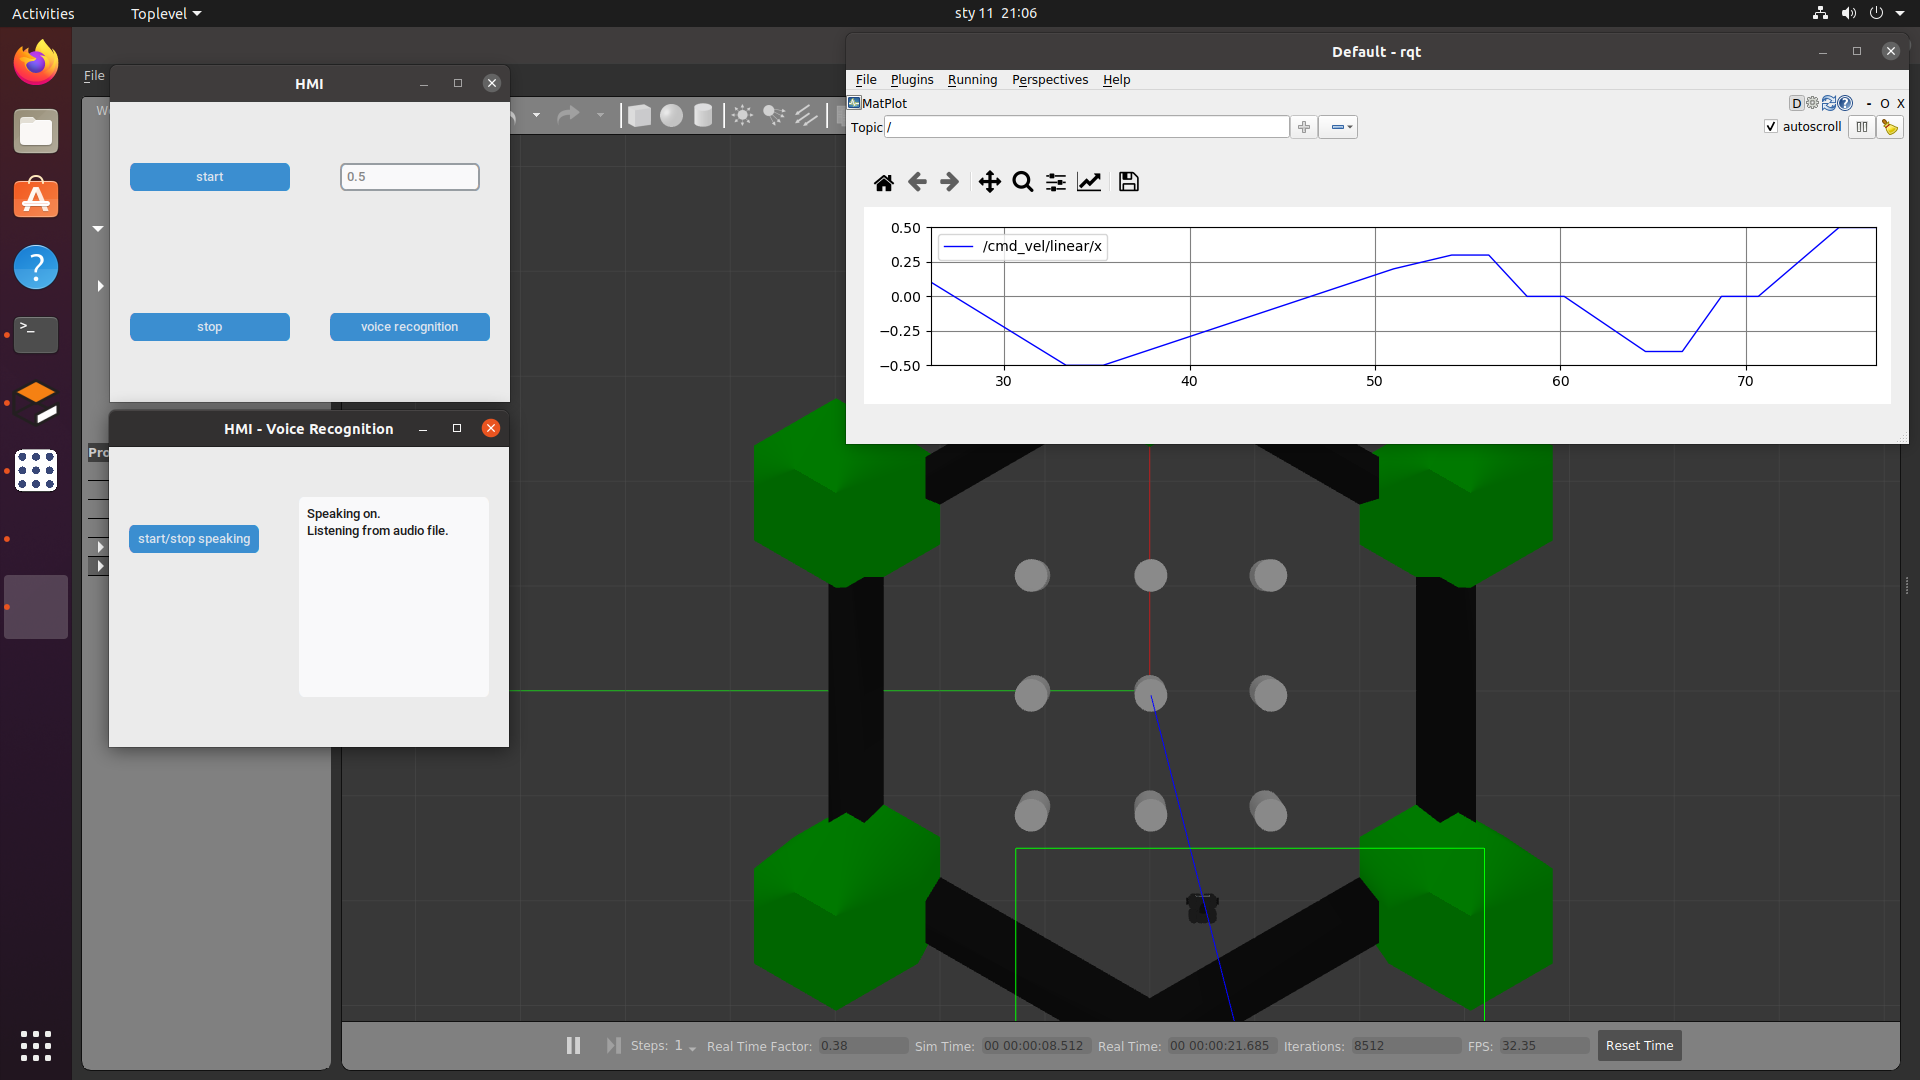
\includegraphics[width=1\linewidth]{files/start.png}
    \captionof{figure}{Widok okna symulacji z panelem do sterowania.}
    \label{fig:start_gazebo}
\end{center}
\vfill

\begin{center}
    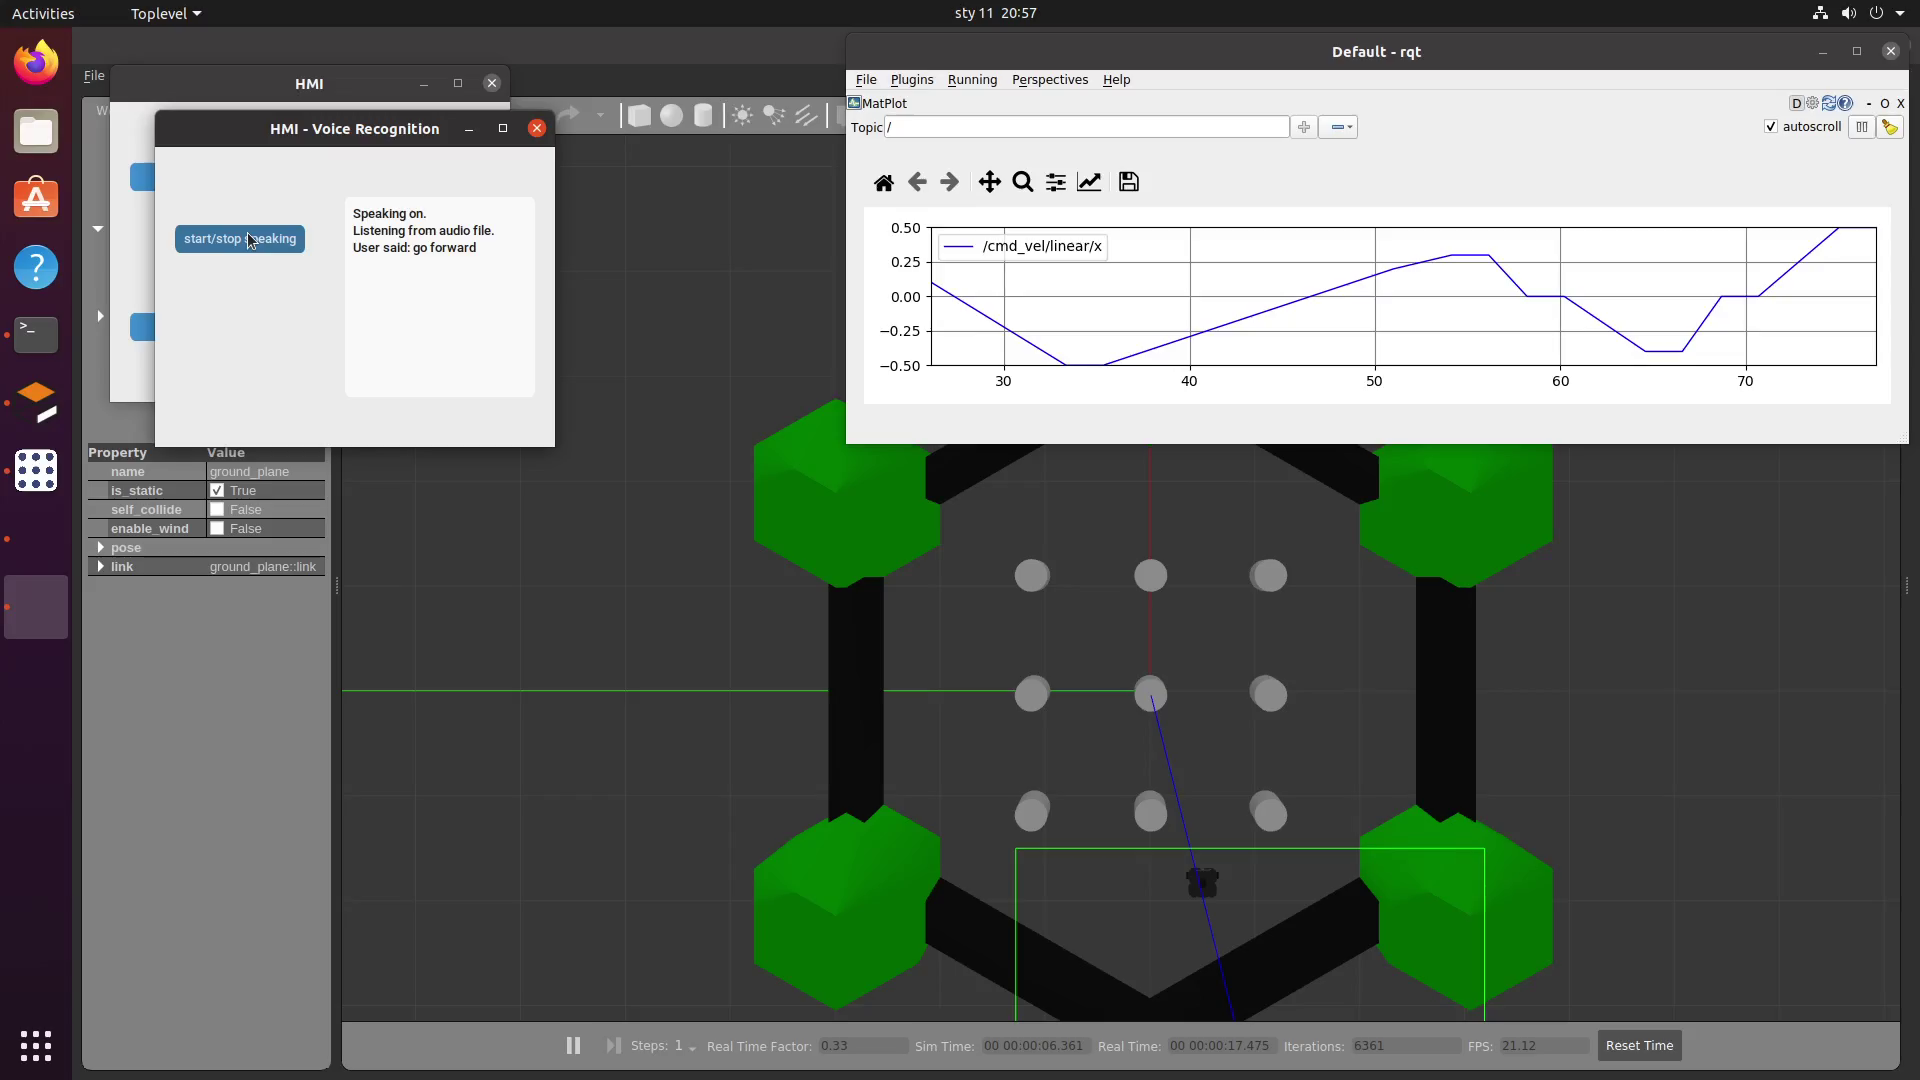
\includegraphics[width=1\linewidth]{files/ruch.png}
    \captionof{figure}{Widok okna symulacji ze sterowanym głosowo robotem.}
    \label{fig:ruch_gazebo}
\end{center}

\begin{center}
    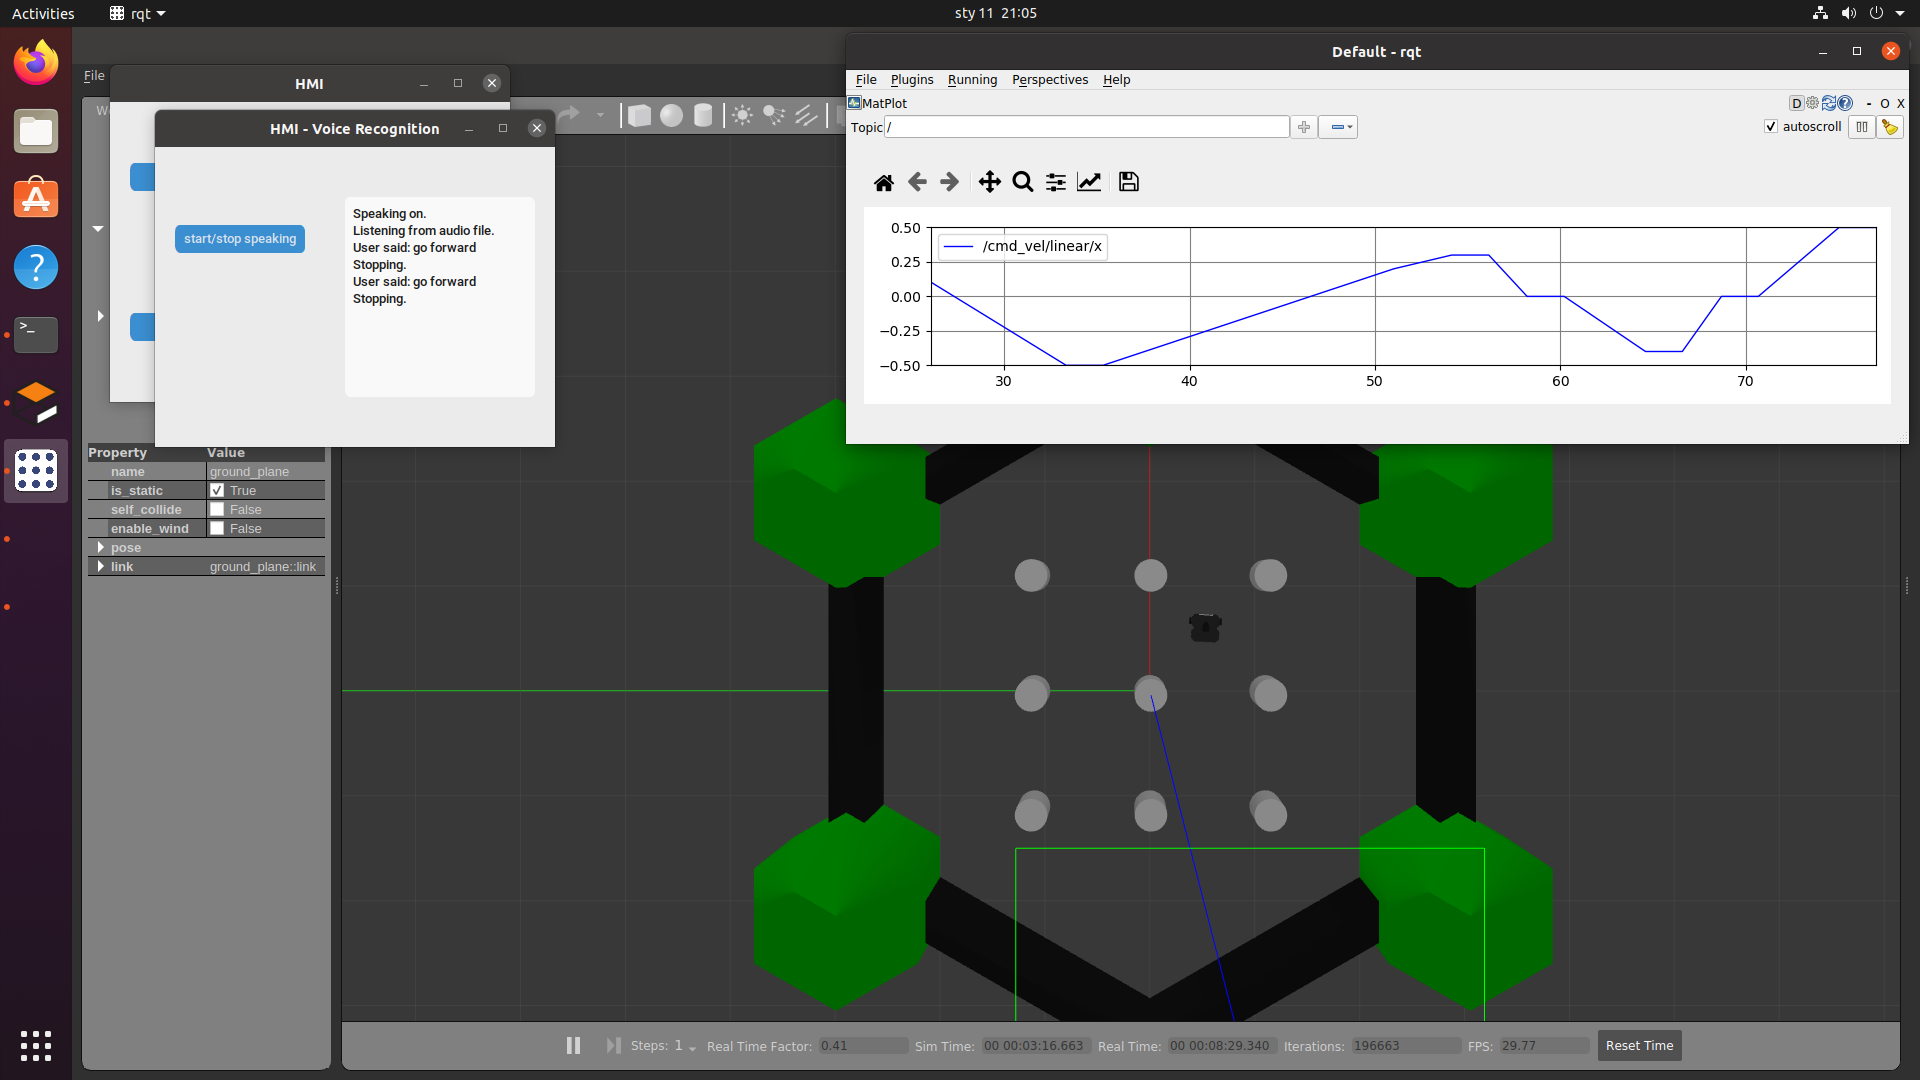
\includegraphics[width=1\linewidth]{files/koniec.png}
    \captionof{figure}{Widok okna symulacji po wykonaniu przez robota sekwencji.}
    \label{fig:koniec_gazebo}
\end{center}

Na Rys. \ref{fig:koniec_gazebo} można zaobserwować sekwencję ruchu wykonaną przez robota, widoczną w oknie informacji zwrotnej panelu. 
%---------------------------------------------------------------------------